\chapter{Introduction}
\label{ch:introduction}
\graphicspath{{figures/ch_1/}}

The statistical modeling of infectious disease data is among the oldest applications of statistics, beginning with Bernoulli's work on smallpox in the 18th century \citep{Bernoulli2004}.
Today, it is an increasingly relevant application of research, due to globalization that enables diseases to spread further and faster, as well as the abundance of relevant data from electronic surveillance systems, social contact and mobility patterns from mobile phones, and genetic sequencing of pathogens.
The importance of this pursuit is apparent when reflecting on the recent COVID-19 pandemic, which resulted in millions of deaths and the largest global recession in nearly a century \citep{whocoronavirus,  zumbrun_2020}.

\section{Epidemic Surveillance Data and Its Applications}
\label{ch_1:sec:epidemic_surveillance_data}

Infectious disease data differs from data used in traditional statistical applications because they are highly dependent in time and space, and are almost always partially observed \citep{held2019handbook}.
People without healthcare access or who do not exhibit disease symptoms may not seek diagnosis, leading to systematic bias and under-reporting in case counts.
Among those who seek diagnosis, their disease status may not be correctly identified, and their results may not be reported to a centralized database.
Even among those who receive a correct diagnosis and whose diagnostic test results are reported, the precise timing of infection, transmission, and recovery are generally unknown.
These factors make inference and forecasting challenging.
For instance, a small outbreak with a high reporting rate may produce similar observed case counts as a large outbreak with a low reporting rate.
% The situation is even more opaque for endemic diseases, where these unreported cases contribute to differing levels of immunity throughout a population.

Infectious disease surveillance data can be reported at a variety of resolutions and used for a variety of tasks.
Some methods are designed to work with detailed data from a specific, relatively small outbreak, while others are more suitable for widespread diseases observed with less detail.
This work is primarily concerned with the latter scenario and uses both passively and actively collected surveillance data.
These data sources traditionally take the form of aggregated counts of incidence data (e.g., new tests, new cases, and new deaths), counts of prevalence data (e.g., the number of hospitalized patients with a disease or the number of people with seropositive tests from a sampled population) at some coarse demographic, spatial, and temporal resolution (e.g., stratified by age and county and documented weekly).
Our work and other recent advances seek to integrate other forms of data into this framework \citep{Rasmussen2011, Tang2022}.

These data and models are vital tools for both inference and forecasting tasks.
One major goal in the inference context is nowcasting, which typically involves estimating the effective reproduction number, \( R_t \), in real time \citep{10.1093/aje/kwt133}.
This parameter is defined as the expected number of secondary cases that arise from a primary case and is influenced by factors inherent to the pathogen, as well as the environmental conditions.
For example, consider the case of a new virus variant emerging in the summer.
The new variant may be inherently more transmissible than the previously circulating strain, driving up the effective reproduction number.
Simultaneously, the warmer weather and school closures work to decrease the effective reproduction number.
Of most concern is the threshold \( R_t = 1 \).
When \( R_t < 1 \), the average primary case produces fewer than one secondary case.
If this is sustained, prevalence will decrease.
When \( R_t > 1 \), the average primary case produces more than one secondary case, leading to an exponential increase in cases.
Other inference tasks involve quantifying the effects of interventions, whether they be pharmaceutical (e.g., vaccination campaigns) or non-pharmaceutical (e.g., mask mandates).
Other inference tasks may be more basic.
For an example, an infectious disease modeler may simply want to infer the true proportion of the population that has been infected with a disease.
Beyond inference, modelers may also be interested in forecasting future disease burden, often with special attention to severe outcomes like hospitalizations and deaths \citep{10.1371/journal.pmed.1003793}.
Relatedly, modelers may consider potential future scenarios to drive public policy by  by answering questions like ``in the presence of a more transmissible variant, how many people do we need to vaccinate to prevent the healthcare system from being overwhelmed?"

In the next section, we provide an overview of surveillance data available to infectious disease modelers to motivate our methodological contributions.

\section{Motivating Examples}
\label{ch_1:sec:motivating_examples}

In Chapter~\ref{ch:content_1}, we work with data originally analyzed by \citet{Kali:2021}.
This data set was collected to estimate the cumulative incidence of SARS-CoV-2 in undiagnosed adults in the United States between May and July 2020.
The data consists of 304 seropositive samples among the 8058 total antibody tests.
The samples are weighted based on a variety of socioeconomic factors. 
 The assay used is estimated to have perfect sensitivity, based on 56 tests on individuals with confirmed SARS-CoV-2 and perfect specificity based on 300 tests on individuals confirmed to not have SARS-CoV-2.

In Chapter~\ref{ch:content_2}, we analyze data from Orange County, California between March 2020 and February 2021.
This data includes case and mortality data provided by Orange County Health Care Agency, including individual-level records of all negative and positive PCR tests during the modeling period.
The aggregated counts of cases, tests, deaths, and test-positivity (cases / tests) are presented in Figure~\ref{ch_1:fig:binned_data_plot}.
This figure is labelled with three periods.
In each period, there is some tension in the trend portrayed by the various data streams, each of which we believe to be reflective of the underlying number of infections.
In the first period, there is a gradual increase in both tests and deaths, a sudden increase in cases, and a gradual decline in test positivity, which is followed by a sudden increase.
In the second period, tests rise slightly, while deaths, cases, and test positivity remain nearly constant.
In the final period, there is a sharp increase and decrease in deaths and test positivity, while tests and cases have a large dip in the middle of this period.
Resolving the conflicting signals between these data streams is the goal of Chapter~\ref{ch:content_2}.
To achieve this goal, we also use data from \citet{Bruckner2021}, a study conducted to estimate the seroprevalence in Orange County from a population-representative sample, which consists of 343 seropositive cases among 2979 tests conducted between July 10 and August 16, 2020.

\begin{figure}
    \centering
    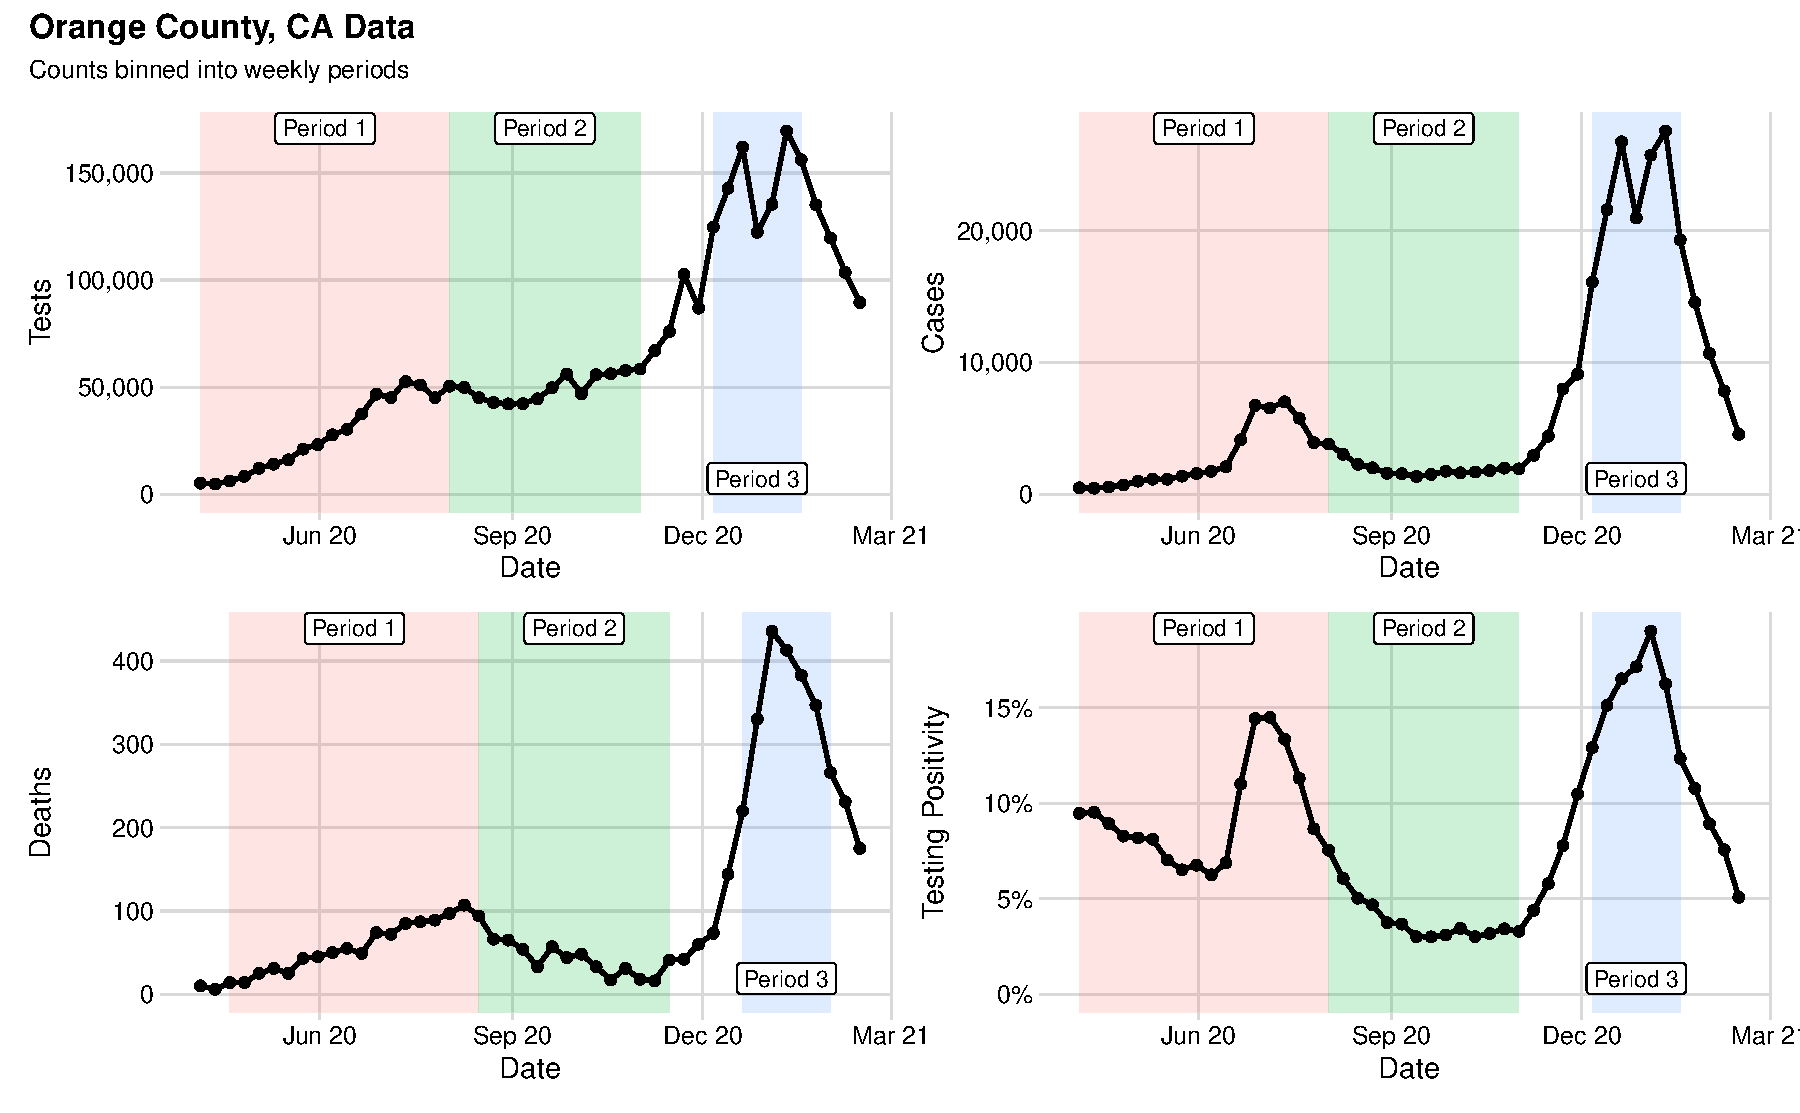
\includegraphics[width=1.0\columnwidth]{binned_data_plot}
    \caption[COVID-19 surveillance data from Orange County, California used in Chapter~\ref{ch:content_2}.]{
    COVID-19 surveillance data from Orange County, California used in Chapter~\ref{ch:content_2}.
    The figure shows weekly counts of tests, cases (positive tests), reported deaths due to COVID-19, as well as testing positivity.
    The distinct periods labelled with different background colors are explained in Section~\ref{ch_1:sec:motivating_examples}.}
    \label{ch_1:fig:binned_data_plot}
\end{figure}

In Chapter~\ref{ch:content_3}, we again analyze data from Orange County, as well as statewide data from California, with a focus on forecasting healthcare demand during the Omicron BA.1 wave of winter 2022. 
Counts of cases, hospital occupancy, ICU occupancy, and deaths are provided to us by the California Department of Public Health.
The counts of virus sequence by variant are provided by the Global Initiative on Sharing All Influenza Data (GISAID) \citep{shu2017gisaid} via Outbreak.info \citep{Gangavarapu2023}.
The aggregated counts of cases, hospital occupancy, ICU occupancy, deaths, and sequence counts of the BA.1 and non-BA.1 variants are presented in Figure~\ref{ch_1:fig:orange_county_binned_data_plot} for Orange County and Figure~\ref{ch_1:fig:california_binned_data_plot} at the statewide level.
The gray highlighted regions indicate the times for which we create forecasts.
The objective of this chapter is to develop a model that uses the proportion of BA.1 sequences to improve forecasting during this time of rapidly changing dynamics.

\begin{figure}
    \centering
    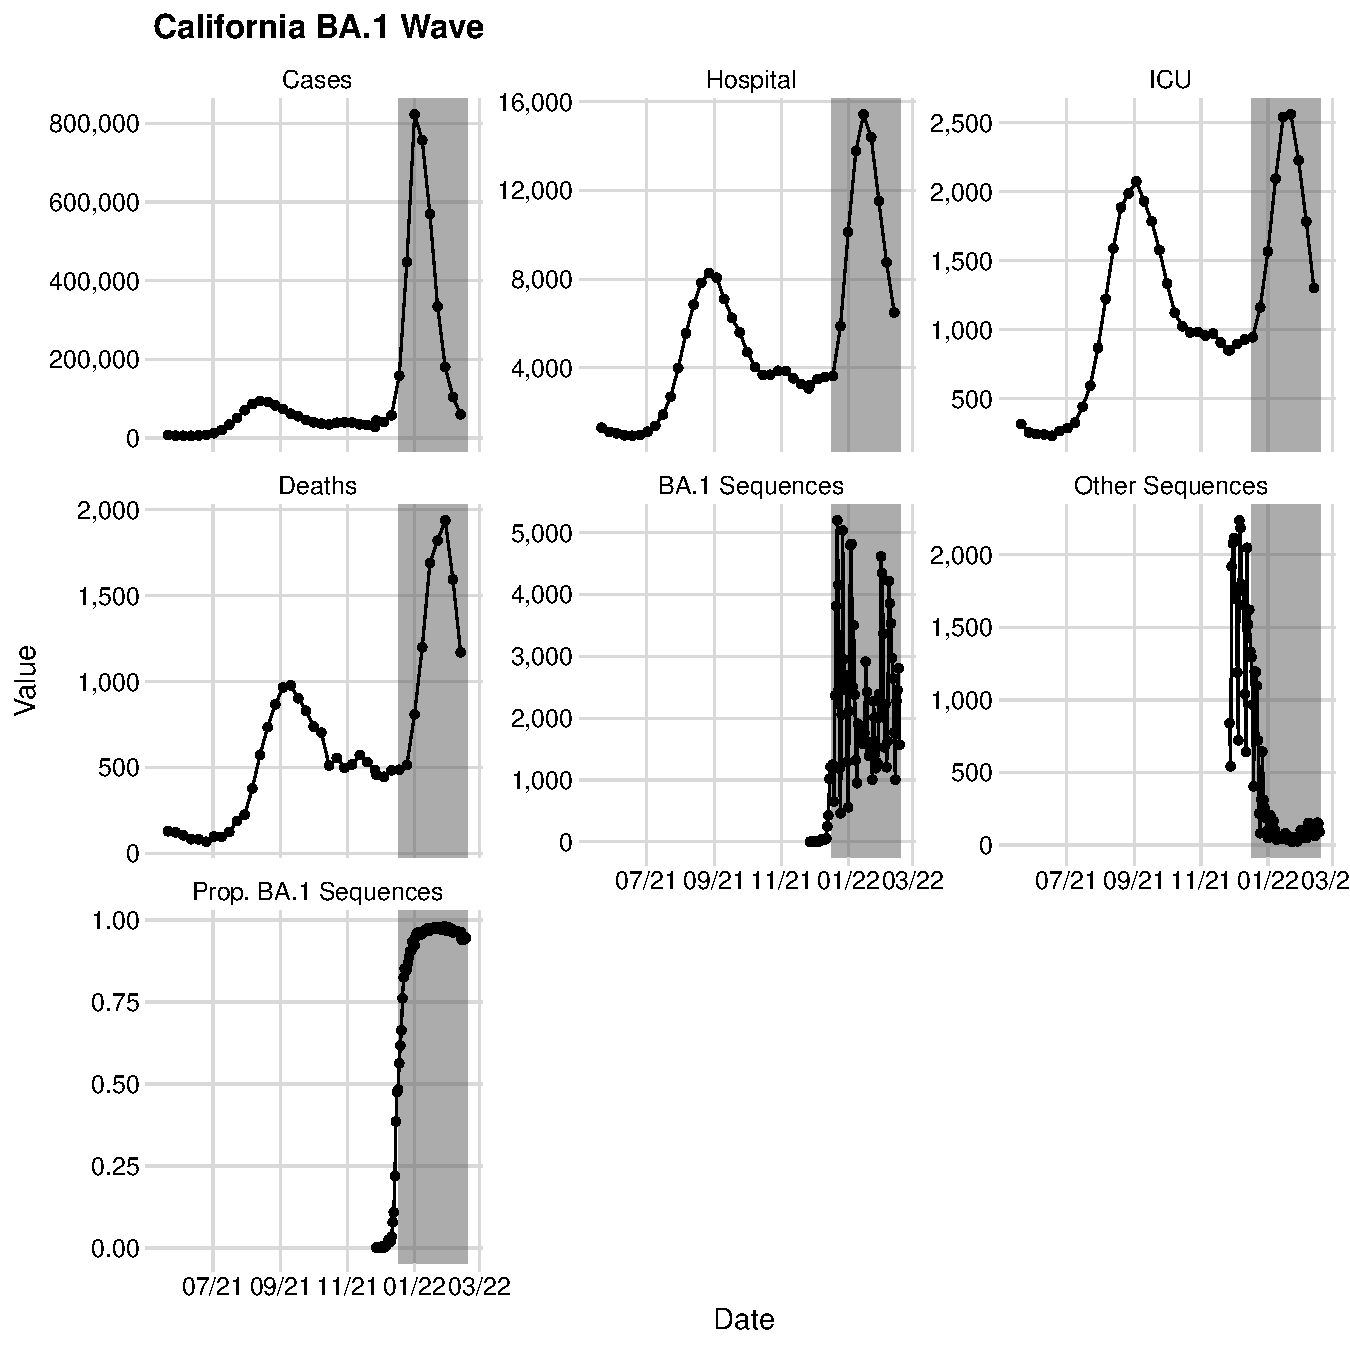
\includegraphics[width=1.0\columnwidth]{figures/ch_5/california_binned_data_plot.pdf}
    \caption[Statewide COVID-19 surveillance data from California used in Chapter~\ref{ch:content_3}.]{
Statewide COVID-19 surveillance data from California used in Chapter~\ref{ch:content_3}.
The plots show weekly counts of cases, hospital and ICU occupancy of patients with COVID-19, reported deaths due to COVID-19, as well as counts of virus sequences for Omicron BA.1 and all lineages, and the proportion of BA.1 lineages.
The gray highlighted regions indicate the times for which we produce forecasts.}
    \label{ch_1:fig:california_binned_data_plot}
\end{figure}

\begin{figure}
    \centering
    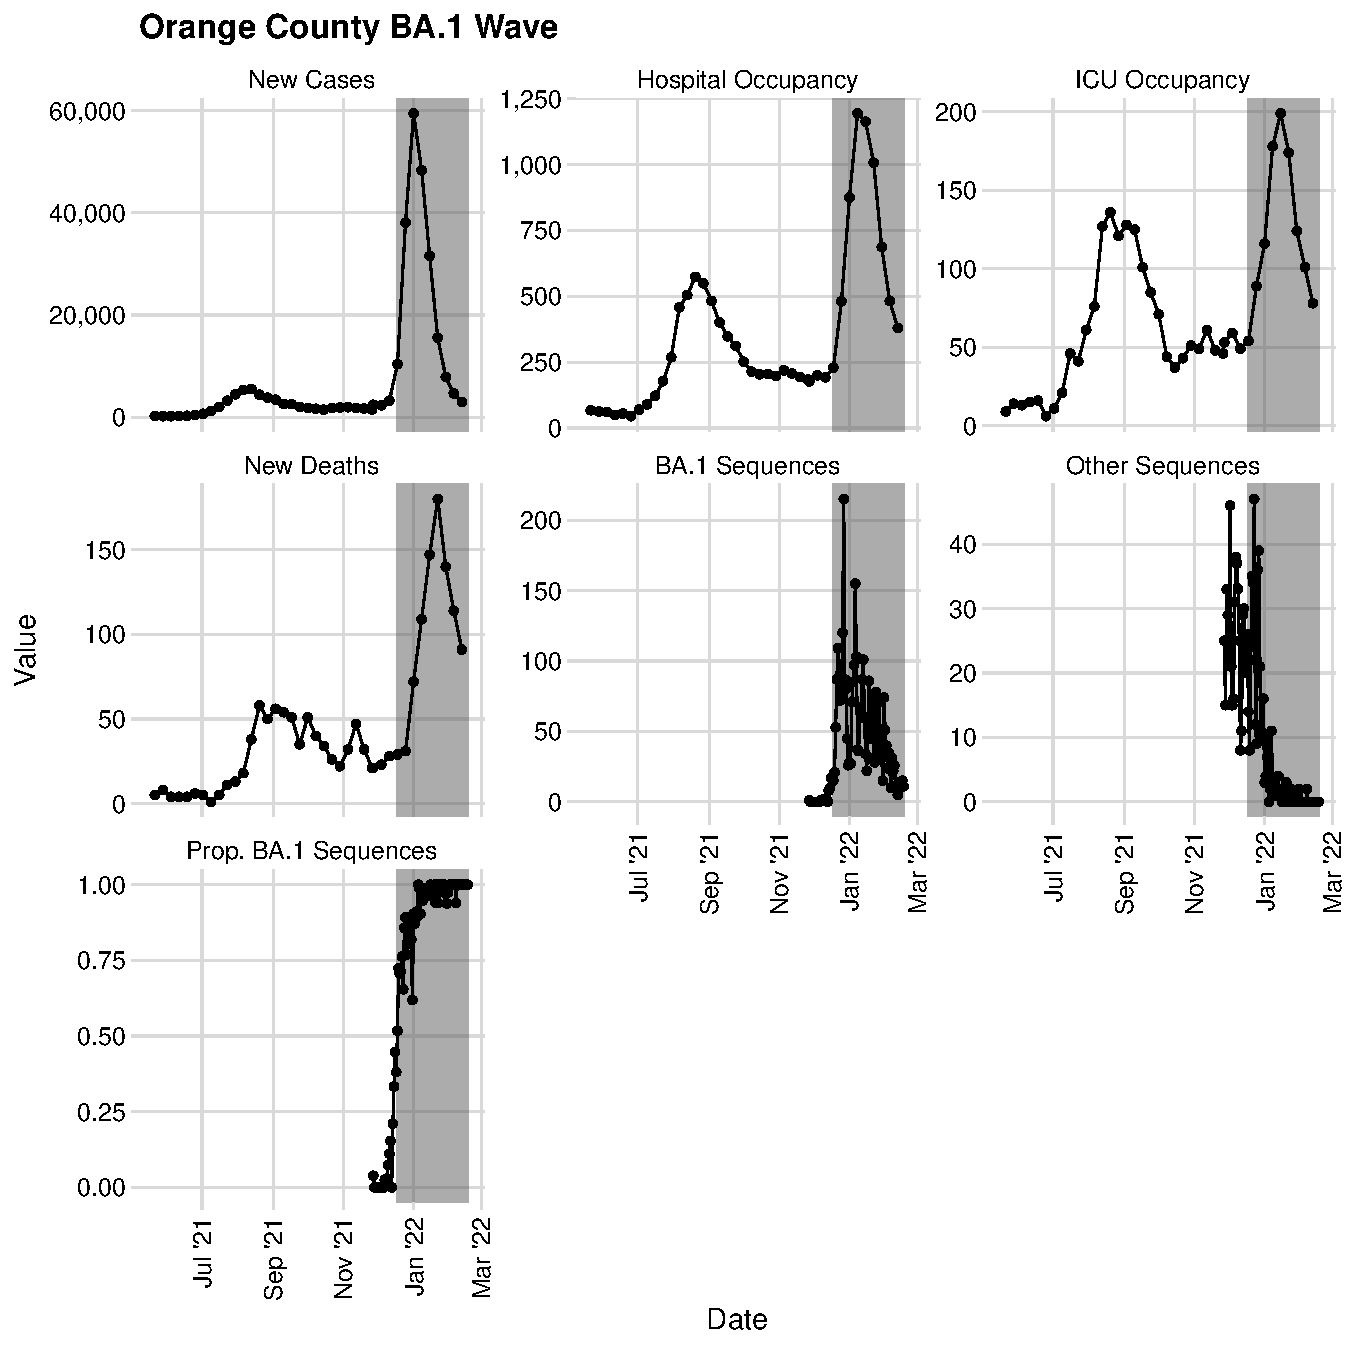
\includegraphics[width=1.0\columnwidth]{figures/ch_5/orange_county_binned_data_plot.pdf}
    \caption[COVID-19 surveillance data from Orange County, California used in Chapter~\ref{ch:content_3}.]{
COVID-19 surveillance data from Orange County, California used in Chapter~\ref{ch:content_3}.
The plots show weekly counts of cases, hospital and ICU occupancy of patients with COVID-19, reported deaths due to COVID-19, as well as counts of virus sequences for Omicron BA.1 and all lineages, and the proportion of BA.1 lineages.
The gray highlighted regions indicate the times for which we produce forecasts.}
    \label{ch_1:fig:orange_county_binned_data_plot}
\end{figure}

\section{Overview of this dissertation}
Chapter~\ref{ch:background} provides background information on areas of statistics essential to understanding the methods proposed and assessed in this dissertation.
The topics covered include mathematical models for the spread of infectious diseases, Bayesian inference and Markov chain Monte Carlo, forecast assessment, and fiducial inference.

In Chapter~\ref{ch:content_1}, we eschew the temporal complications of analyzing infectious disease data and focus on issues of sampling schemes and diagnostic test accuracy.
While there are established methods for estimating disease prevalence with associated confidence intervals for complex surveys with perfect assays and simple random sample surveys with imperfect assays, the case of complex surveys with imperfect assays remains relatively unexplored.
We develop and study new methods for this setting.
The new methods use the melding method to combine gamma intervals for directly standardized rates and established adjustments for imperfect assays by estimating sensitivity and specificity.
One of the new methods appears to have at least nominal coverage in all simulated scenarios.
We compare our new methods to established methods in special cases (complex surveys with perfect
assays or simple surveys with imperfect assays).
In some simulations, our methods appear to guarantee coverage, while competing methods have much lower than nominal coverage, especially when overall prevalence is very low.
In other settings, our methods are shown to have higher than nominal coverage.
We apply our method to a seroprevalence survey of SARS-CoV-2 in undiagnosed adults in the United States between May and July 2020 and find that our methods estimate less overall prevalence than a method which does not account for imperfections in the assay.

In Chapter~\ref{ch:content_2}, we turn our attention to the temporal dynamics of infectious diseases in the presence of changing policy and behavior.
Mechanistic models fit to streaming surveillance data are critical for understanding the transmission dynamics of an outbreak as it unfolds in real-time.
However, transmission model parameter estimation can be imprecise, and sometimes even impossible because surveillance data are noisy and not informative about all aspects of the mechanistic model.
To partially overcome this obstacle, Bayesian models have been proposed to integrate multiple surveillance data streams. 
We devise a modeling framework for integrating SARS-CoV-2 diagnostics test and mortality time series data, as well as seroprevalence data from cross-sectional studies, and tested the importance of individual data streams for both inference and forecasting.
Importantly, our model for incidence data accounts for changes in the total number of tests performed.
We apply our Bayesian data integration method to COVID-19 surveillance data collected in Orange County, California between March 2020 and February 2021 and find that 32--72\% of the Orange County residents experienced SARS-CoV-2 infection by mid-January, 2021.
Despite this high number of infections, our results suggest that the abrupt end of the winter surge in January 2021 was due to both behavioral changes and a high level of accumulated natural immunity.

In Chapter~\ref{ch:content_3}, we work in a similar setting as Chapter~\ref{ch:content_2}, but where the changing disease dynamics are due to novel disease variants, rather than changing policy and behavior.
In this chapter, we are primarily concerned with forecasting, rather than inference.
Accurate forecasting of epidemic surges is an important tool for public health agencies to make informed decisions about interventions and resource allocation.
Forecasting is particularly challenging when a new variant arises, which may result in increased transmissibility, severity, or immune evasion, leading to surges in cases, hospitalizations, or deaths.
To improve forecasting in these scenarios, we propose a way to integrate raw counts of variant sequences into a Bayesian compartmental model.
We assume that the observed count of sequences of a novel variant has a beta-binomial distribution whose mean is a product of the total number of observed genetic sequences and the proportion of the infectious population with the novel variant.
We then model the average duration of immunity as a flexible function of this proportion.
We evaluate our method in a simulation study wherein novel variants become dominant at varying rates and to data from the Omicron wave in Orange County, California and the state of California as a whole.
In these assessments, our model is shown to have superior forecasting performance and is especially better at forecasting the timing and magnitude of the peak hospital occupancy, a metric crucial for public health officers and hospital managers making staffing decisions.

We conclude with a summary of our work in Chapter~\ref{ch:discussion} and discuss opportunities for future research in inference and forecasting using infectious disease surveillance data.

\label{ch_1:sec:thesis_contributions}

%touch on traditional methods (SIR Model)

% This is an example using the \LaTeX{} template for UCI theses and
% dissertation documents \cite{uci-thesis-latex}. Figure
% \ref{fig:sourcecode} is just for illustration purposes, as is Table
% \ref{tab:coordinates}.

% \begin{figure}
% \begin{verbatim}
% #include <iostream>
% int main(int argc, char** argv) {
%   std::cout << "Hello World." << std::endl;
%   return 0;
% }
% \end{verbatim}
%   \caption{Example source code.}
%   \label{fig:sourcecode}
% \end{figure}

% \section{Background}

% Lorem ipsum dolor sit amet, consectetur adipisicing elit, sed do
% eiusmod tempor incididunt ut labore et dolore magna aliqua. Ut enim ad
% minim veniam, quis nostrud exercitation ullamco laboris nisi ut
% aliquip ex ea commodo consequat. Duis aute irure dolor in
% reprehenderit in voluptate velit esse cillum dolore eu fugiat nulla
% pariatur. Excepteur sint occaecat cupidatat non proident, sunt in
% culpa qui officia deserunt mollit anim id est laborum.

% \begin{table}
%   \centering
%   \begin{tabular}{|rr|r|}
%     \hline
%     $x$ & $y$ & $z$ \\
%     \hline
%     14 & 12 & -2 \\
%     0 & 33 & -25 \\
%     -3 & 11 & 22 \\
%     4 & 4 & 6 \\
%     \hline
%   \end{tabular}
%   \caption{Example coordinates.}
%   \label{tab:coordinates}
% \end{table}

% Lorem ipsum dolor sit amet, consectetur adipisicing elit, sed do
% eiusmod tempor incididunt ut labore et dolore magna aliqua. Ut enim ad
% minim veniam, quis nostrud exercitation ullamco laboris nisi ut
% aliquip ex ea commodo consequat. Duis aute irure dolor in
% reprehenderit in voluptate velit esse cillum dolore eu fugiat nulla
% pariatur. Excepteur sint occaecat cupidatat non proident, sunt in
% culpa qui officia deserunt mollit anim id est laborum.


%%% Local Variables: ***
%%% mode: latex ***
%%% TeX-master: "thesis.tex" ***
%%% End: ***
